% ----------------------------------------------------------------------------
\section{Features}
This section describes which features are supported by the chat protocol.
Figure \ref{features-technologies} gives a quick overview of how the
features relate to the used technologies.
\begin{figure}
    \centering
    \caption{Features and Technologies}
    \label{features-technologies}
    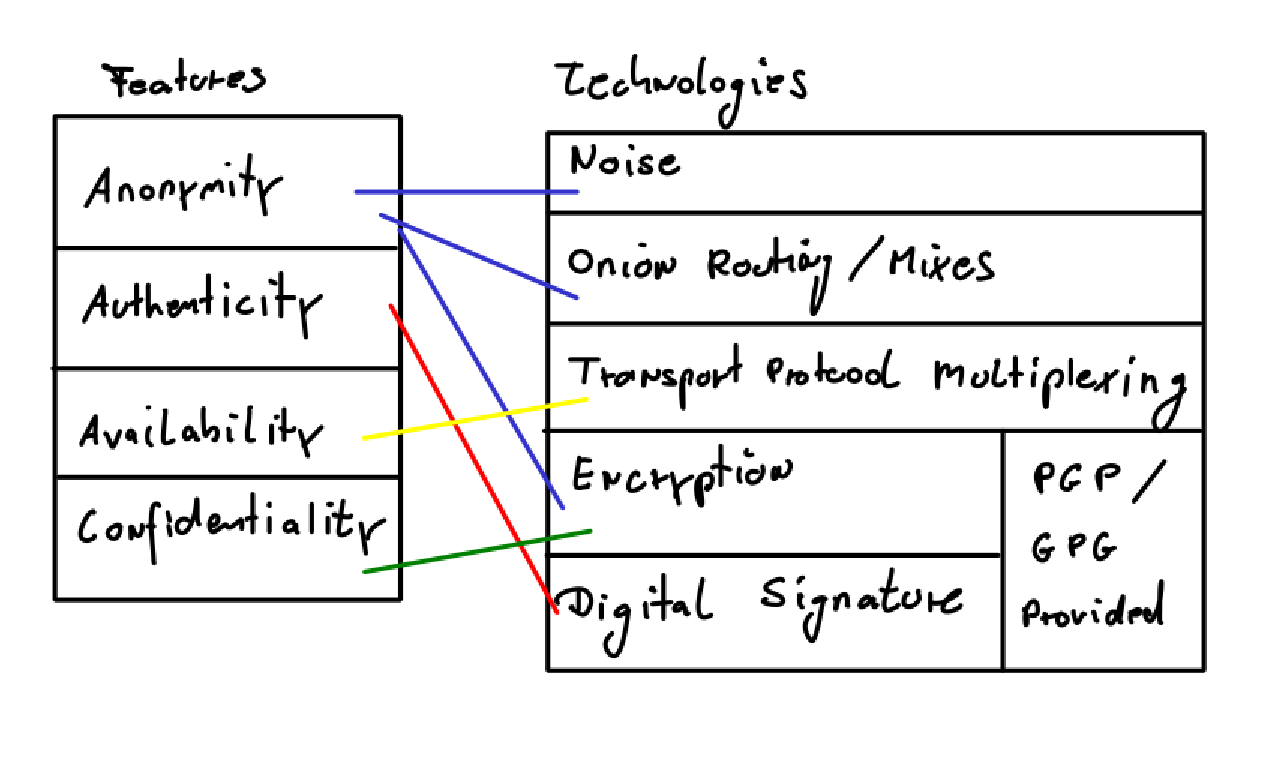
\includegraphics[scale=0.8]{features-technologies.eps}
\end{figure}
% ----------------------------------------------------------------------------
\subsection{Anonymity}
One of the main objectives of this thesis is to provide a chat system that
hides who is talking to whom (\textit{Sender-Receiver Anonymity}). 
In practise there are limits on the degree of anonymity that can be reached.


If an attacker controls all hosts that are 
part of the chat network, it is impossible to guarantee anonymity.

Thus the implementation should support be resistent against a high percentage
of attacker nodes in the network.

Level of anonymity in theory - nodes

Winning chances in Lotto are expressed like this:
$$P_r = \frac{{\binom{6}{r}}{\binom{N-6}{6-r}}}{{\binom{N}{6}}}, r \in \{0, \ldots, 6\}$$

To remove anonymity, all peers in a route, which are not the 
sender and the receiver have to be compromised.
Depending on the number of hosts in a network (number of possible
numbers in lotto) and on the number of hosts in a specific route
(number of correct numbers in lotto), the de-anonymisation
probalities (lotto: winning probabilities) are shown in table
\ref{deanontable}

%\begin{longtable}{|c|c|c|c|c|c|c|c|c|}
\begin{longtable}{|c|c|c|c|c|c|}
\caption{De-Anonymisation Probablities (for one packet)}
\label{deanontable}\\
\hline
\textbf{Peers in network /} & \textbf{$10$} & \textbf{$10^2$} & \textbf{$10^3$} & \textbf{$10^4$} & \textbf{$10^5$} \\
\textbf{Proxy peers} & & & & & \\
\hline
\textbf{1} & 1:10 & 1:100 & 1:1000 & 1:10000 & 1:100000\\
\hline
\textbf{2} & 1:45 & 1:4950 & 1:499500 & 1:4.9995e+07 & 1:4.99995e+09\\
\hline
\textbf{3} & 1:120 & 1:161700 & 1:1.66167e+08 & 1:1.66617e+11 & 1:1.66662e+14\\
\hline
\textbf{4} & 1:210 & 1:3.92122e+06 & 1:4.14171e+10 & 1:4.16417e+14 & 1:4.16642e+18\\
\hline
\textbf{5} & 1:252 & 1:7.52875e+07 & 1:8.25029e+12 & 1:8.325e+17 & 1:8.3325e+22\\
\hline
\textbf{6} & 1:210 & 1:1.19205e+09 & 1:1.36817e+15 & 1:1.38681e+21 & 1:1.38868e+27\\
\hline
\textbf{7} & 1:120 & 1:1.60076e+10 & 1:1.94281e+17 & 1:1.97996e+24 & 1:1.98371e+31\\
\hline
\textbf{8} & 1:45 & 1:1.86088e+11 & 1:2.41151e+19 & 1:2.47322e+27 & 1:2.47946e+35\\
\hline
\textbf{9} & 1:10 & 1:1.90223e+12 & 1:2.65802e+21 & 1:2.74583e+30 & 1:2.75474e+39\\
\hline
\textbf{10} & 1:1 & 1:1.73103e+13 & 1:2.6341e+23 & 1:2.74336e+33 & 1:2.75449e+43\\
\hline
\end{longtable}
To support a high chance of not hitting the attackers peers and thus
avoiding de-anonymisation, the number
of peers in the network as well as the number of proxy peers should be
increased as much as possible. The number of peers in the network are
depending on how many peers are actually using the network. This can be
increased to a certain degree by adding artificial peers.
The number of proxy peers cannot be increades infinitely, because every
additional proxy peers adds an amount of time to the latency until the
message arrives.

hoi, hoi ... latency counts afterwards. but includes reaction time.

% ----------------------------------------------------------------------------
\subsection{Authenticity}
Digital signatures provide methods to ensure that a given message
was composed by a given public key and that the content has not been
modified.
% ----------------------------------------------------------------------------
\subsection{Confidentiality}
The process of encryption protects data and thus ensures the
confidentiality of a message.
% ----------------------------------------------------------------------------
\subsection{Availability}
% ----------------------------------------------------------------------------
\subsection{Non security related features}
This chat protocol version supports only direct chat as opposed to
multi user / group chat.


